
\chapter{Linear transformations}

\index{linear transformation}
\index{function}

A \textbf{linear transformation} is actually just another spin on matrix-vector
multiplication. It's also yet another way to view a matrix as a
\textit{function}. Back on p.~\pageref{matrixIsFunction}, I made the point that
instead of drawing numbers in a grid, you could view a matrix itself as a
function, where the input is an ordered pair (row and column numbers) and the
output is the element at that entry. In this chapter, we explore a deeper and
richer interpretation of a matrix as a \textit{different} sort of function.

\section{Transforming one vector into another}

Recall how matrix-vector multiplication works. We'll write it notationally as
$A \cdot \overrightarrow{\textbf{x}} = \overrightarrow{\textbf{y}}$, where
$\overrightarrow{\textbf{y}}$ is the result of the multiplication. Now we could
think about the operation like this:

\begin{compactitem}
\item $A$ is a ``function'' of sorts, which works on vectors to produce other
vectors.
\item $\overrightarrow{\textbf{x}}$ is the input vector we give to that
function.
\item $\overrightarrow{\textbf{y}}$ is the function's output (result).
\end{compactitem}

\index{machine}
We're thinking of $A$ as a long-lasting, reusable thing, whereas
$\overrightarrow{\textbf{x}}$ and $\overrightarrow{\textbf{y}}$ stand for the
temporary inputs \& outputs that we give to $A$ and compute on the fly. My
mental image is of $A$ as a machine, $\overrightarrow{\textbf{x}}$ as the raw
materials we might feed to the machine, and $\overrightarrow{\textbf{y}}$ as
the machine's completed work.

One natural question is: ``what is the domain, and the range, of this $A$
function?'' That depends on $A$'s dimensions. Suppose it's a $3\times 2$
matrix:

\vspace{-.15in}
\begin{align*}
\begin{bmatrix}
2 & 3 \\
1 & -4 \\
0 & 5 \\
\end{bmatrix} \cdot \textrm{\Large ?} = \textrm{\Large ?}
\end{align*}
\vspace{-.15in}

\index{domain}
\index{codomain}
We know from the rules of matrix-vector multiplication
(p.~\pageref{matVecRules}) that the first question mark has to be a
\textbf{2}-dimensional column vector, else the operation is impossible. And we
know that the output will be a \textbf{3}-dimensional column vector. This means
that the domain of the $A$ ``function'' is 2-d vectors and the codomain is 3-d
vectors. Most commonly, this is written as follows:

\vspace{-.15in}
\begin{align*}
A : \mathbb{R}^2 \rightarrow \mathbb{R}^3.
\end{align*}
\vspace{-.15in}

Remember from \textit{A Cool, Brisk Walk} that the $\mathbb{R}$ sign means
``the set of real numbers.'' When we say ``$\mathbb{R}^2$'' we're saying ``the
set of vectors with two real-numbered entries.'' And $\mathbb{R}^3$ is the set
of \textit{three}-dimensional real vectors, \textit{etc.}

Put all together, the purpose of our $A$ matrix is to map each two-dimensional
vector to a particular three-dimensional vector. For instance, it maps the 2-d
vector $[\ 2 \ \ 1\ ]$ to:

\vspace{-.15in}
\begin{align*}
\begin{bmatrix}
2 & 3 \\
1 & -4 \\
0 & 5 \\
\end{bmatrix} \cdot 
\begin{bmatrix}
2 \\ 1 \\
\end{bmatrix} =
\begin{bmatrix}
7 \\ -2 \\ 5 \\
\end{bmatrix}.
\end{align*}
\vspace{-.15in}

The particular vector it chooses seems kind of random so far, and indeed this
first example is just pulled from the air. Normally there will be some
``meaning'' to the transformation.

\index{linear map}

By the way, a linear transformation is sometimes called a \textbf{linear map}
because it performs this ``mapping'' operation, like a function does. The two
terms (linear transformation and linear map) are exact synonyms.

\subsection{Meaningful examples}

Before we go any further, let's at least show that this is useful. I'm going to
create a machine (matrix) $B$ (for ``Body,'' sort of) that transforms certain
4-dimensional vectors into 2-dimensional ones. Here it is:

\vspace{-.15in}
\begin{align*}
B = 
\begin{bmatrix}
12 & 1 & 0 & 0 \\
0 & 0 & 2.2 & 0 \\
\end{bmatrix}.
\end{align*}
\vspace{-.15in}

The kind of input this matrix/function is intended to act on a vector such as
$\overrightarrow{\textbf{stephen}}$, which is structured like this:

\vspace{-.3in} 
\begin{align*}
\begin{matrix*}[r]
\textrm{\small{height: whole feet}} \rightarrow \\
\textrm{\small{height: extra inches}} \rightarrow \\
\textrm{\small{weight: kilograms}} \rightarrow \\
\textrm{\small{shoe size}} \rightarrow \\
\end{matrix*}
\begin{bmatrix}
6 \\ 2 \\ 95.5 \\ 13 \\
\end{bmatrix}
\end{align*}
\vspace{-.15in}

This rather revealing vector contains some of my vital bodily stats. I'm 6'2"
tall, and hence don't fit on airplanes; I weigh too much at 95.5 kg; and I wear
an impossible-to-fit 13 shoe (13AAA, actually; blame my mom's side of the
family).

Now what happens when we feed this to the $B$ machine?

\vspace{-.15in}
\begin{align*}
B \cdot \overrightarrow{\textbf{stephen}} =
\begin{bmatrix}
12 & 1 & 0 & 0 \\
0 & 0 & 2.2 & 0 \\
\end{bmatrix} \cdot
\begin{bmatrix}
6 \\ 2 \\ 95.5 \\ 13 \\
\end{bmatrix} =
\begin{bmatrix}
74 \\ 210 \\
\end{bmatrix}
\begin{matrix*}[l]
\leftarrow \textrm{\small{height in inches}} \\
\leftarrow \textrm{\small{weight in pounds}} \\
\end{matrix*}
\end{align*}
\vspace{-.15in}

This matrix-vector multiplication produces a 2-element vector, since

\vspace{-.15in}
\begin{align*}
B : \mathbb{R}^4 \rightarrow \mathbb{R}^2.
\end{align*}
\vspace{-.15in}

The first element is my height in total inches, and the second element is my
weight in pounds. And it will do so for every person whose 4-dimensional vector
it's multiplied by. Interestingly, the shoe size of the input vector plays no
role in the value of the output vector, because there are zero elements at both
$B_{0,3}$ and $B_{1,3}$. And that's okay.

\smallskip
\index{BMI (body-mass index)}

By the way, you might think about expanding this example to calculate something
more complex like a BMI (body-mass index). After all, BMI is a straightforward
function of a person's weight and height\footnote{(Mine's about 27, which puts
me in the ``obese'' range I'm sorry to say.)}, as you might know:

\vspace{-.15in}
\begin{align*}
\textrm{BMI} = 703 \times \frac{\textrm{weights (lbs)}}{\textrm{height (in)}^2}.
\end{align*}
\vspace{-.15in}


However, it turns out this is \textit{impossible} to do with a linear
transformation. The reason is it's not linear! The only operations that can be
included in a linear transformation are dot products, because that's what
matrix-vector multiplication \textit{is}. So for each element of our output
vector, we can (1) take the elements of the input vector, (2) multiply each of
them by any constant we like, and (3) add up the results. The BMI formula, by
contrast, requires us to \textit{divide} one of our inputs by another, and in
fact requires us to \textit{square} that second input before dividing. These
are both decidedly non-linear operations that cannot be expressed with a
matrix.

This may seem limiting, and in a way it is, but keep in mind two things. First,
there are lots and lots and lots of common operations that \textit{are} linear,
and all of those come under our power in this book on linear algebra. Second,
when we do have linear operations, we can take advantage of all kinds of
computational simplifications and analytical tricks, so concentrating on the
linear case is most definitely worth our time.

\bigskip

\index{stock prices}
Here's a second example. Suppose I have the following odd-looking matrix $S$
(for ``stocks,'' sort of):

\vspace{-.15in}
\begin{align*}
S =
\begin{bmatrix}
0 & 1 & 0 \\
0 & .69 & 0 \\
0 & 111.1 & 0 \\
0 & .88 & 0 \\
0 & 6.48 & 0 \\
0 & 17.37 & 0 \\
\end{bmatrix}
\end{align*}
\vspace{-.15in}

What does it do? Well, it's designed for us to feed it vectors representing
Wall Street stocks, like so:

\index{McDonald's}
\vspace{-.3in} 
\begin{align*}
\overrightarrow{\textbf{mcdonalds}} =
\begin{bmatrix}
1965 \\ 183.52 \\ 2606707 \\
\end{bmatrix}
\begin{matrix*}[l]
\leftarrow\textrm{\small{year founded}} \\
\leftarrow\textrm{\small{current share price}} \\
\leftarrow\textrm{\small{trading volume}} \\
\end{matrix*}
\end{align*}
\vspace{-.15in}

The result of multiplying $S$ by this kind of vector is to give us a
convenient list of the McDonald's current stock price in various currencies:

\vspace{-.3in} 
\begin{align*}
S \cdot \overrightarrow{\textbf{mcdonalds}} =
%\begin{bmatrix}
%0 & 1 & 0 \\
%0 & .69 & 0 \\
%0 & 111.1 & 0 \\
%0 & .88 & 0 \\
%0 & 6.48 & 0 \\
%0 & 17.37 & 0 \\
%\end{bmatrix} \cdot
%\begin{bmatrix}
%1965 \\ 183.52 \\ 2606707 \\
%\end{bmatrix} =
\begin{bmatrix}
183.52 \\ 126.93 \\ 20389.10 \\ 161.50 \\ 1189.21 \\ 3187.74 \\
\end{bmatrix}
\begin{matrix*}[l]
\leftarrow\textrm{\small{\EyesDollar \ (U.S. dollars)}} \\
\leftarrow\textrm{\small{\pounds \ (British pounds sterling)}} \\
\leftarrow\textrm{\small{\textyen \ (Japanese Yen)}} \\
\leftarrow\textrm{\small{\EURtm \ (Euros)}} \\
\leftarrow\textrm{\small{\textyen \ (Chinese Yuan)}} \\
\leftarrow\textrm{\small{\textpeso \ (Mexican Pesos)}} \\
\end{matrix*}
\end{align*}
\vspace{-.15in}

Again, the $S$ matrix is simply ignoring the information we don't care about,
and that's okay. It's still a function:

\vspace{-.15in}
\begin{align*}
S : \mathbb{R}^3 \rightarrow \mathbb{R}^6.
\end{align*}
\vspace{-.15in}


\section{Linear operators}

\index{square matrix}
\index{linear operator}

So every matrix gives us a linear transformation, no matter its shape. But if
the matrix is \textit{square}, we use a special name for the linear
transformation it carries out: a \textbf{linear operator}.

A matrix being square, of course, would imply that the input vectors and the
output vectors (or the domain and codomain, if you prefer) are the \textit{same
dimension}: the function will map vectors in $\mathbb{R}^3$ to other vectors in
$\mathbb{R}^3$, for instance, or from $\mathbb{R}^{81}$ to $\mathbb{R}^{81}$.

Let's restrict our attention for the moment to just two dimensions, and see
what effect certain $2\times 2$ linear operator matrices have on the vectors
they act upon.

\begin{figure}[hb]
\centering
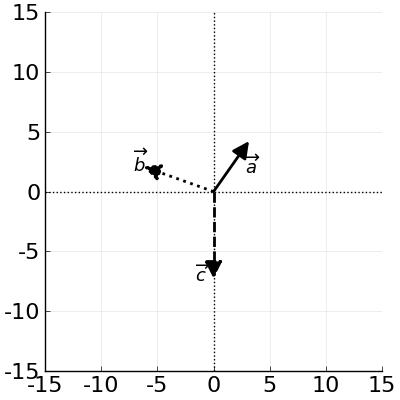
\includegraphics[width=0.44\textwidth]{preoperators.png}
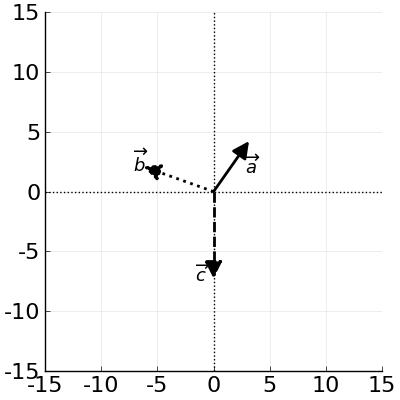
\includegraphics[width=0.44\textwidth]{preoperators.png}
\caption[.]{Three vectors, and their transformations under the linear operator 
{\scriptsize $\begin{bmatrix} 1 & 0 \\ 0 & 1 \\ \end{bmatrix}$.}}
\label{fig:identityOp}
\end{figure}

\index{identity matrix}

We'll have three guinea pig vectors, which are:
$\overrightarrow{\textbf{a}} = [\ 3\ \ 4\ ]$ (solid),
$\overrightarrow{\textbf{b}} = [\ -6\ \ 2\ ]$ (dotted), and
$\overrightarrow{\textbf{c}} = [\ 0\ \ -7\ ]$ (dashed). They're plotted in the
left half of Figure~\ref{fig:identityOp}. First, we'll try the identity matrix,
which you'll remember in two dimensions is simply:

\vspace{-.15in}
\begin{align*}
I_2 =
\begin{bmatrix}
1 & 0 \\
0 & 1 \\
\end{bmatrix}
\end{align*}
\vspace{-.15in}


Let's multiply our three guinea pigs by this matrix to transform them:

\vspace{-.15in}
\begin{align*}
I_2 \cdot \overrightarrow{\textbf{a}} &=
\begin{bmatrix}
1 & 0 \\
0 & 1 \\
\end{bmatrix} \cdot
\begin{bmatrix}
3 \\ 4 \\
\end{bmatrix} =
\begin{bmatrix}
3 \\ 4 \\
\end{bmatrix}.
\end{align*}

\vspace{-.15in}
\begin{align*}
I_2 \cdot \overrightarrow{\textbf{b}} &=
\begin{bmatrix}
1 & 0 \\
0 & 1 \\
\end{bmatrix} \cdot
\begin{bmatrix}
-6 \\ 2 \\
\end{bmatrix} =
\begin{bmatrix}
-6 \\ 2 \\
\end{bmatrix}.
\end{align*}

\vspace{-.15in}
\begin{align*}
I_2 \cdot \overrightarrow{\textbf{c}} &=
\begin{bmatrix}
1 & 0 \\
0 & 1 \\
\end{bmatrix} \cdot
\begin{bmatrix}
0 \\ -7 \\
\end{bmatrix} =
\begin{bmatrix}
0 \\ -7 \\
\end{bmatrix}.
\end{align*}
\vspace{-.15in}

The effect, you'll agree, is underwhelming. Double-check my math, and convince
yourself that \textit{the function of the identity matrix is to convert a
vector into itself!} This is why it's called the ``identity'' matrix, in fact.
The ``identity element'' of addition is 0, which means if you add anything to
zero, you get your number back as an answer. The identity element of
multiplication is 1, of course. And fun fact, the identity \textit{matrix} is
the matrix {\tiny $\begin{bmatrix} 1 & 0 \\ 0 & 1 \\ \end{bmatrix}$}.

The right half of Figure~\ref{fig:identityOp} illustrates this boring fact:
under the identity matrix's linear operator, all three vectors look exactly the
same after the transformation.

\medskip

K, let's shake things up a bit then. Let's try this operator:

\vspace{-.15in}
\begin{align*}
S_{v=2} =
\begin{bmatrix}
1 & 0 \\
0 & 2 \\
\end{bmatrix}.
\end{align*}
\vspace{-.15in}

I'll reveal why I chose $S_{v=2}$ as the name of this matrix in a moment.
Notice that it is the same as $I_2$ except for the 2 in the bottom-right
corner. What does it do when it maps vectors? Let's give it a shot:

\vspace{-.15in}
\begin{align*}
S_{v=2} \cdot \overrightarrow{\textbf{a}} &=
\begin{bmatrix}
1 & 0 \\
0 & 2 \\
\end{bmatrix} \cdot
\begin{bmatrix}
3 \\ 4 \\
\end{bmatrix} =
\begin{bmatrix}
3 \\ 8 \\
\end{bmatrix},
\end{align*}

\vspace{-.15in}
\begin{align*}
S_{v=2} \cdot \overrightarrow{\textbf{b}} &=
\begin{bmatrix}
1 & 0 \\
0 & 2 \\
\end{bmatrix} \cdot
\begin{bmatrix}
-6 \\ 2 \\
\end{bmatrix} =
\begin{bmatrix}
-6 \\ 4 \\
\end{bmatrix},
\end{align*}

\vspace{-.15in}
\begin{align*}
S_{v=2} \cdot \overrightarrow{\textbf{c}} &=
\begin{bmatrix}
1 & 0 \\
0 & 2 \\
\end{bmatrix} \cdot
\begin{bmatrix}
0 \\ -7 \\
\end{bmatrix} =
\begin{bmatrix}
0 \\ -14 \\
\end{bmatrix}.
\end{align*}
\vspace{-.15in}

\begin{figure}[ht]
\centering
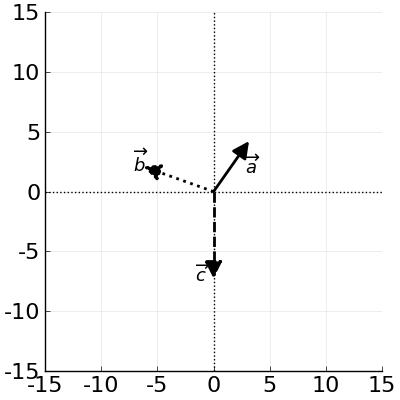
\includegraphics[width=0.44\textwidth]{preoperators.png}
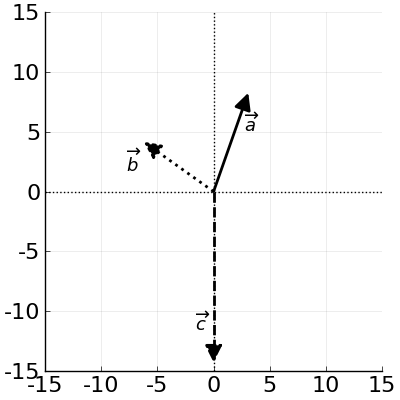
\includegraphics[width=0.44\textwidth]{vertstretchop.png}
\caption[.]{Three vectors, and their transformations under the linear operator 
{\scriptsize $\begin{bmatrix} 1 & 0 \\ 0 & 2 \\ \end{bmatrix}$.}}
\label{fig:vertstretchop}
\end{figure}

Can you see what it did in Figure~\ref{fig:vertstretchop}? It
\textit{stretched all the points vertically by a factor of 2.} In other words,
every vector is now pointing at a point twice as far from the $x$-axis. This is
why I chose the name $S_{v=2}$ -- it stands for ``\textbf{S}tretch
\textbf{v}ertically by a factor of \textbf{2}.''

\pagebreak

Playing on the same theme, we can try:

\vspace{-.15in}
\begin{align*}
S_{v=\frac{1}{2},h=2\frac{1}{2}} =
\begin{bmatrix}
2\frac{1}{2} & 0 \\
0 & \frac{1}{2} \\
\end{bmatrix}.
\end{align*}
\vspace{-.15in}

Let's see what this bad boy does to our vectors:

\vspace{-.15in}
\begin{align*}
S_{v=\frac{1}{2},h=2\frac{1}{2}} \cdot \overrightarrow{\textbf{a}} &=
\begin{bmatrix}
2\frac{1}{2} & 0 \\
0 & \frac{1}{2} \\
\end{bmatrix} \cdot
\begin{bmatrix}
3 \\ 4 \\
\end{bmatrix} =
\begin{bmatrix}
7\frac{1}{2} \\ 2 \\
\end{bmatrix},
\end{align*}

\vspace{-.15in}
\begin{align*}
S_{v=\frac{1}{2},h=2\frac{1}{2}} \cdot \overrightarrow{\textbf{b}} &=
\begin{bmatrix}
2\frac{1}{2} & 0 \\
0 & \frac{1}{2} \\
\end{bmatrix} \cdot
\begin{bmatrix}
-6 \\ 2 \\
\end{bmatrix} =
\begin{bmatrix}
-15 \\ 1 \\
\end{bmatrix}.
\end{align*}

\vspace{-.15in}
\begin{align*}
S_{v=\frac{1}{2},h=2\frac{1}{2}} \cdot \overrightarrow{\textbf{c}} &=
\begin{bmatrix}
2\frac{1}{2} & 0 \\
0 & \frac{1}{2} \\
\end{bmatrix} \cdot
\begin{bmatrix}
0 \\ -7 \\
\end{bmatrix} =
\begin{bmatrix}
0 \\ -3.5 \\
\end{bmatrix}.
\end{align*}
\vspace{-.15in}

\begin{figure}[hb]
\centering
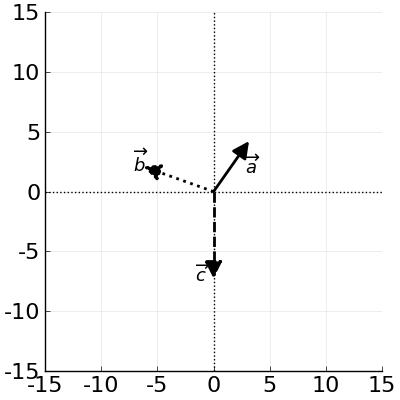
\includegraphics[width=0.44\textwidth]{preoperators.png}
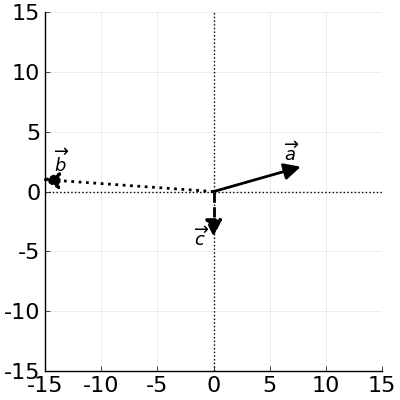
\includegraphics[width=0.44\textwidth]{stretchSquishOp.png}
\caption[.]{Three vectors, and their transformations under the linear operator 
{\scriptsize $\begin{bmatrix} 2\frac{1}{2} & 0 \\ 0 & \frac{1}{2} \\
\end{bmatrix}$,} which is a bit like being simultaneously sat on by two
mirror-image giants.}
\label{fig:stretchSquishOp}
\end{figure}
\index{giant butts}

Figure~\ref{fig:stretchSquishOp} shows the results. Our vectors have been both
stretched and squished: stretched wide away horizontally from the $y$-axis, and
squished towards the $x$-axis. It's like a giant sat down on the $x$-axis --
and his evil twin giant below him sat ``up'' on the $x$-axis, so that their
butts nearly met in the middle. All the blades of grass on both sides of the
axis were nearly smashed under the composite load. (Btw, if this visual image
isn't doing it for you, by all means disregard it.)




% [ -1 0 ; 0 1 ]  maps [ 4 -1 ] to [ -4 -1 ]. reflects horizontally across y-axis

% [ 0 -1 ; 1 0 ]  maps [ 4 1 ] to [ -1 4 ], [ 1, -1 ] to [ 1 1 ],
%                      [ -2 -4 ] to [ 4 -2 ]. Rotation 90 deg CCW.
%
% [ sqrt(2)/2  - sqrt(2)/2 ; sqrt(2)/2  sqrt(2)/2 ]
%                 maps [2 3] to ...    Rotation 45 deg CCW.

% In general, to rotate by theta, use [ cos q   -sin q  ;  sin q   cos q ]

% Movie CGI, video games, use all of this

% Foreshadowing: Multiple operators all strung together!
% Scaling [ 4 0 ; 0 4 ]  x  rotation[ sqrt(2) ]  x  flip[ -1 0 ; 0 1 ]
